\documentclass[titlepage, 11pt]{article}
\usepackage[utf8]{inputenc}     			% UTF8 encoding
\usepackage[margin=1in]{geometry}     		% margins 

\usepackage{hyperref} 						% href
\usepackage{graphicx}
\usepackage[font=small,labelfont=bf]{caption} % Required for specifying captions to tables and figures
\usepackage{verbatimbox}


\title{
	\textbf{Mini Project 1} \\
	Machine learning (CS582), MIU \thanks{Instructor: Anthony Sander}
}

\author{Baraa Mousa Noufal \and Ivan Krasowski Bissio}
\date{\today}

\begin{document}
\maketitle
\tableofcontents

\begin{abstract}
	\addcontentsline{toc}{section}{Abstract}
	
\begin{center}
    \begin{minipage}{0.85\textwidth}
        Machine Learning models are used to predict data of interest using known data as input.
        For an airline, it is useful to be able to predict if a passenger will be satisfied with their flight, and what to improve in case for those passengers who won't.
        Classifiers are the Machine Learning resource for said predictions.\\
        The goal of this study is to test several classifiers for predicting Airline Passengers Satisfaction, show their performance and optimize them, in order to choose the best of them.
    \end{minipage}
\end{center}
\end{abstract}

\section{About the Dataset}
% Something about the dataset. What it is, where to find it (link), why we chose it...
The chosen dataset collects information about \href{https://www.kaggle.com/binaryjoker/airline-passenger-satisfaction/download}{Airline Passenger Satisfaction}.
We opted for this dataset because it had a lot of entries (almost 130000), many columns (including 4 categorical) and it was oriented to a binary classification problem ('satisfied' vs. 'neutral or dissatisfied').

\subsection{EDA: Exploratory Data Analysis}
\begin{itemize}
	\item The dataset collects multiple features related to each passenger-flight, including labels for whether the passenger was satisfied with the flight or not.
	\item It has 24 columns (22 + id + result).
	\item Id column is dropped (it would add weight).
	% TODO: add reference to missing values treatment
	\item Observation: the only column with null values is 'arrival\_delay\_in\_minutes', with 393 missing values.
	\item Categorical columns: 4
	\subitem \underline{Features and possible values}: Gender (2), customer\_type (2), type\_of\_travel (2), customer\_class (3)
	\subitem \underline{Decision}: use one-hot encoding in all of them (none of them is a clear candidate for being weighted)
	\item Looking for strong correlations: pairwise correlation function to check if two features show strong correlation.
	\subitem NOTE: 'satisfaction' (the label we will try to predict) is not strongly correlated ($>$0.7) with any of the other features. 
	\subitem \emph{arrival\_delay\_in\_minutes} and \emph{departure\_delay\_in\_minutes} have the highest correlation rate (0.965291), which semantically makes sense; all other variables are less than 75\% correlated.
	\subitem \begin{center}
		\captionsetup{type=figure}
		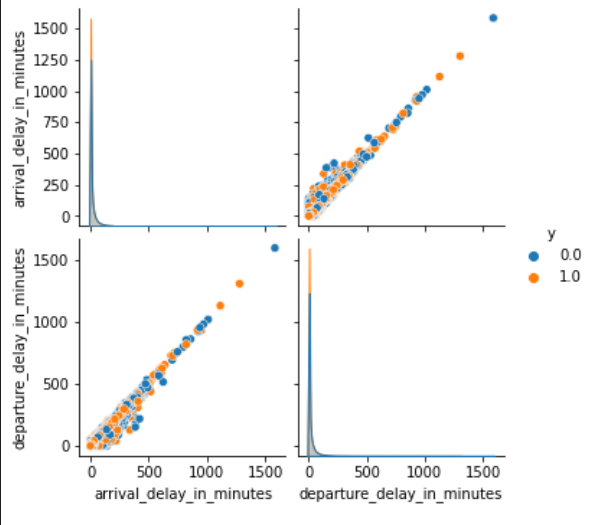
\includegraphics[width=250px]{correlation.png}
		\captionof{figure}{Correlation between most-correlated features}
	\end{center}
\end{itemize}

\subsection{Data Preparation}
\begin{enumerate}
	\item X: all table except id and result ('satisfaction') columns;  y: 'satisfaction' column
	\item Since the arrival\_delay feature is highly correlated with the departure\_delay feature, and the missing values are not that many (393 out of 129879: ~0.03\%), we decide to remove the column.
	\item We see there are 4 categorical features, with no more than 3 unique values each. So, given that none of them is a clear candidate for being weighted, we decide to use one-hot encoding in all of them.
	\item Finally, we split X and y for training and validating, following a ratio of 80\%/20\% (the dataset is large enough).
	\subitem \emph{Variables: \textbf{X\_train, X\_val, y\_train, y\_val}}
\end{enumerate}

\section{Models}
\subsection{KNN}
\subsubsection{Presentation}
KNearestNeighbors algorithm works by holding instances of training data and classifying by issuing a majority vote across "k" nearest neighbor of each point as to which class it belongs.

\subsubsection{Defining Parameters}
The data for training and validating is already defined by the Data Preparation step (80\% train, 20\% validation).\\
The representative parameter for KNN is \emph{n\_neighbors}: The number of neighboring instances taking part in the classification vote.\\

We trained the model on the default parameters (n\_neighbors=5) and achieved a 77\% accuracy on validation data.\\
We then attempted to tune the \emph{n\_neighbors} parameter using GridSearch across a range of values, it turned out the best value found by GridSearch for \emph{n\_neighbors} was 5 as well.\\
Next, we plotted the model score over a similar range, but scoring on the test dataset (rather than GridSearch).
\begin{center}
    \captionsetup{type=figure}
    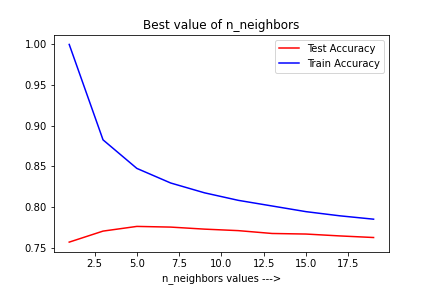
\includegraphics[width=250px]{knn_complexity.png}
    \captionof{figure}{Complexity Curve: \emph{n\_neighbors} value for KNN}
\end{center}
Observing the plot, it shows the same result as the validation accuracy starts to dip after \emph{n\_neighbors}=5.

\subsubsection{Model Evaluation}
Setting \emph{n\_neighbors}=5, we train another KNNClassifier and plot its learning curve as the data increases.
\begin{center}
    \captionsetup{type=figure}
    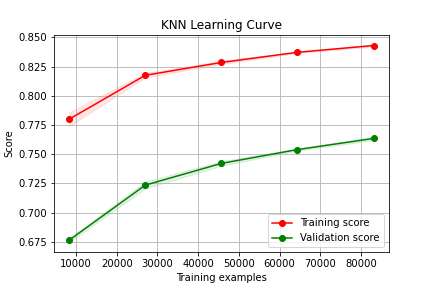
\includegraphics[width=250px]{learning_curve_knn.png}
    \captionof{figure}{Learning Curve for KNN}
\end{center}
Plot shows high variance but decreasing bias with more training data.

\subsection{Decision Tree}
% \subsubsection{Presentation}
% \subsubsection{Training}
% \subsubsection{Validation}
% ... some more subsubsections (like results)

\subsection{Support Machine Vector}
\subsubsection{Presentation}
Support Vector Machines are a model of supervised learning.\\
In summary, the model finds the hyperplane (kernel) that maximizes the Margin of Safety for classifying.

\subsubsection{Defining Parameters}
The data for training and validating is already defined by the Data Preparation step (80\% train, 20\% validation).\\
Representative parameters for the model are \emph{gamma} and \emph{C}
\begin{itemize}
    \item \underline{gamma}: kernel coefficient
    \item \underline{C}: regularization parameter (higher C, higher variance)
\end{itemize}
We train the following values for the \emph{gamma} parameter: [0.001, 0.01, 0.03, 0.05, 0.08, 0.1, 0.5]
To improve the predictions, we regularize the data using a StandardScaler (removes the mean and scales to unit variance)
The training error and the validation error for each value allow us to plot a Complexity Curve, to select the optimal value fo the parameter.
\begin{center}
    \captionsetup{type=figure}
    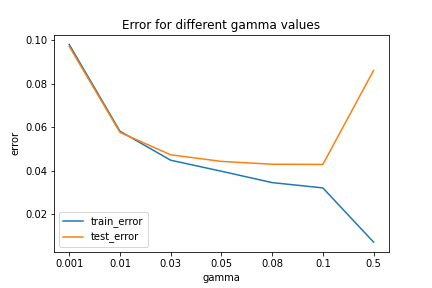
\includegraphics[width=250px]{comp_curve_svm_gamma.png}
    \captionof{figure}{Complexity Curve: \emph{gamma} value for SVM}
\end{center}
By observing the plot, we determine that the best value for gamma is 0.03\\
We train the following values for the \emph{C} parameter: [0.02, 0.2, 0.8, 1.2, 2, 5, 10]\\
Again, we regularize the data using a StandardScaler (removes the mean and scales to unit variance)\\
The training error and the validation error for each value allow us to plot a new Complexity Curve, to select the optimal value fo the parameter.
\begin{center}
    \captionsetup{type=figure}
    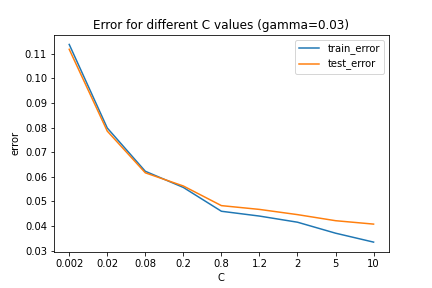
\includegraphics[width=250px]{comp_curve_svm_C.png}
    \captionof{figure}{Complexity Curve: \emph{C} value for SVM (\emph{gamma}=0.03)}
\end{center}
By observing the plot, we determine that the best value for C is 0.8

\subsubsection{Model Evaluation}
Chosen the parameters: (\emph{gamma}=0.03, \emph{C}=0.8), a learning curve shows us the training and validation scores for different data sizes.\\
This way, we are able to say that the score is bounded below 95\%, and the model doesn't seem to continue learning after 65000/70000 training rows.
\begin{center}
    \captionsetup{type=figure}
    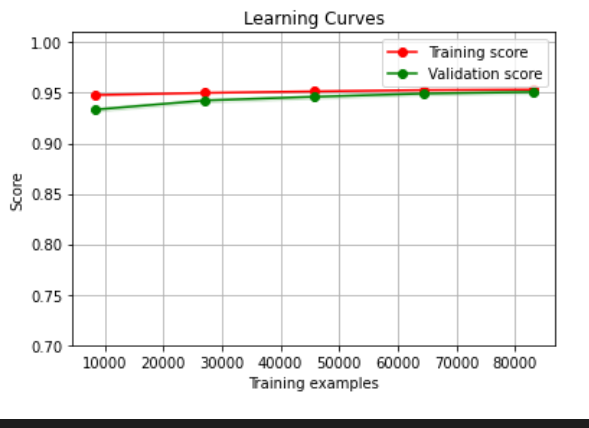
\includegraphics[width=250px]{learning_curve_svm.png}
    \captionof{figure}{Learning Curve for SVM}
\end{center}


\subsection{Neural Network}
\subsubsection{Presentation}
Neural Networks (or Multilayer Perceptrons) are a model of supervised learning, represented by composed non-linear functions.\\
\begin{center}
    \captionsetup{type=figure}
    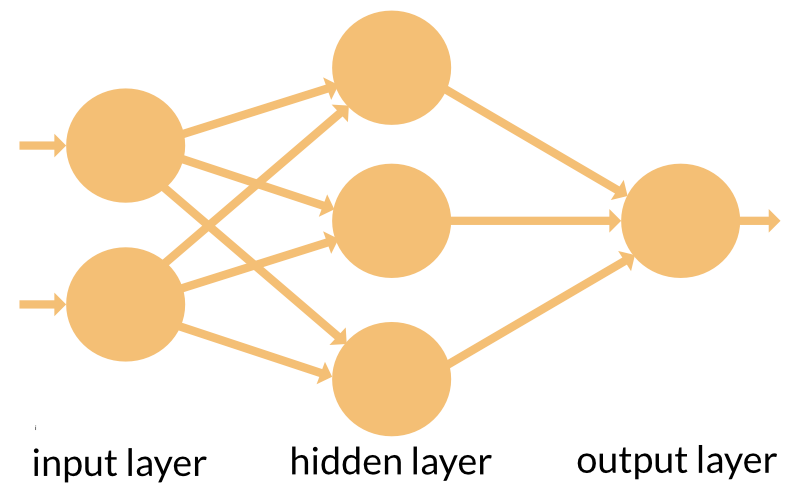
\includegraphics[width=250px]{mlp.png}
    \captionof{figure}{Multilayer Perceptron / Neural Network}\footnote{https://appliedgo.net/perceptron/}
\end{center}
They consist of "neurons", each of which represents a non-linearity, divided in layers, each of which depends on the previous (the first one, on the input data) and is crucial for the next one (the last one gives the output)\\
They can be seen as a function, whose interface is defined by the "input layer" (the first layer) and the "output layer" (the result).\\
All layers between the input layer and the output layer are "hidden layers".\\
A Neural Network makes its predictions after having its parameters (weights) trained with labeled example data (train data)

\subsubsection{Defining Hyperparameters}
The data for training and validating is already defined by the Data Preparation step (80\% train, 20\% validation).\\
Representative hyperparameters (different from the parameters to be trained) for the model are \emph{alpha} and \emph{learning\_rate}
\begin{itemize}
    \item \underline{alpha}: regularization parameter (L2 penalty).
    \item \underline{learning\_rate}: parameter for controlling the step size when updating the weights.
\end{itemize}
A Grid Search is used for getting the best combination of parameters (alpha, learning\_rate) for the input and the model.\\
Values used for \emph{alpha}: [0.001, 0.005, 0.01, 0.05, 0.1]\\
Values used for \emph{learning\_rate}: [0.001, 0.005, 0.01, 0.05, 0.1]
\begin{center}
    \captionsetup{type=figure}
    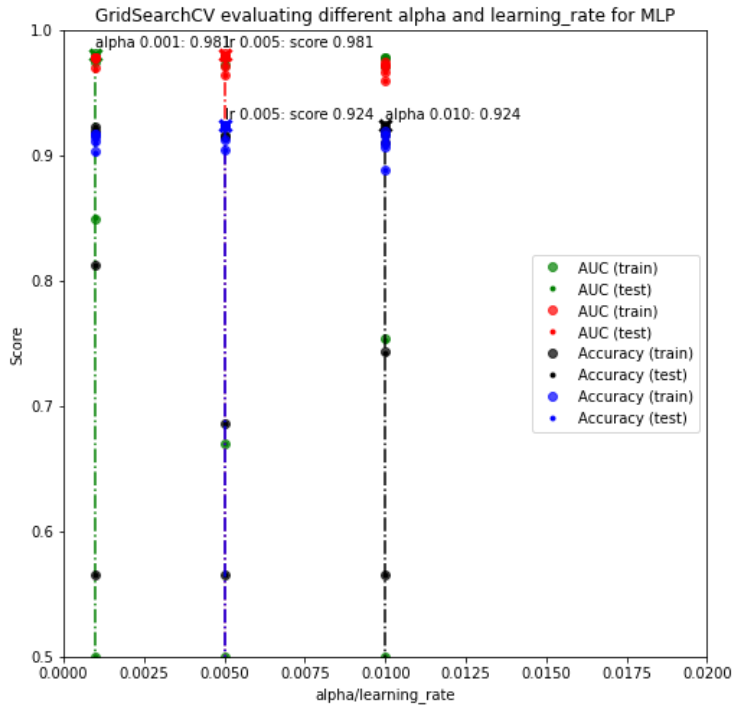
\includegraphics[width=250px]{grid_search_nn.png}
    \captionof{figure}{Grid Search results}
\end{center}
Observable on the plot, and also obtainable by requesting the \emph{grid\_search.best\_params\_}, the best values for the hyperparameters are:
\begin{itemize}
    \item \underline{alpha}: 0.001
    \item \underline{learning\_rate}: 0.005
\end{itemize}

\subsubsection{Model Evaluation}
Chosen the parameters: (\emph{alpha}=0.001, \emph{learning\_rate}=0.005), a learning curve shows us the training and validation scores for different data sizes.\\
This way, we are able to say that the model seems to continue learning after 90000 training rows.
\begin{center}
    \captionsetup{type=figure}
    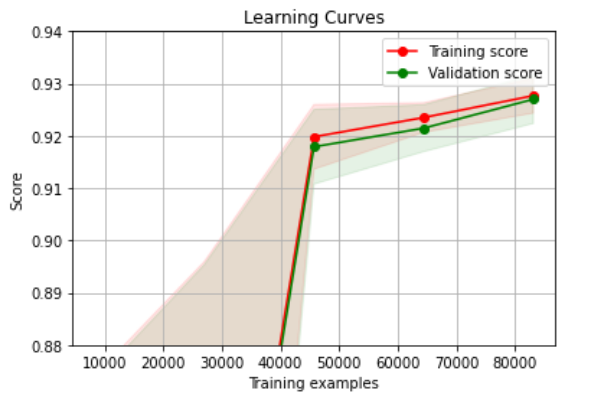
\includegraphics[width=250px]{learning_curve_mlp.png}
    \captionof{figure}{Learning Curve for MLP}
\end{center}


\subsection{Model 5}
\subsubsection{Presentation}
Stochastic Gradient Descent Classifier is an optimization technique to train other classification models, depending on chosen loss function it can be equivalent to an SVM or Logistic Regression models, it is particularly useful for large and sparse data.

\subsubsection{Defining Parameters}
The data for training and validating is already defined by the Data Preparation step (80\% train, 20\% validation).\\
Representative parameters for the model are \emph{max\_iter}, \emph{loss} and \emph{alpha}.
\begin{itemize}
    \item \underline{max\_iter}: stopping criterion, the algorithm can stop before, but never after this number of iterations.
    \item \underline{loss}: loss function, "hinge" is equivalent to a linear SVM, "log" is logistic regression.
    \item \underline{alpha}: regularization parameter (higher alpha, higher variance)
\end{itemize}
We trained \emph{alpha} over a logarithmically decreasing range [1, 0.1, 0.001...10**-7], \emph{max\_iter} over the range [10000, 100000] increasing 10000 per step, as well as across both "hinge" and "log" loss functions.\\
GridSearch was used with those ranges to determine best values for the hyperparameters, it was found to be alpha=0.01, loss=hinge, and  max\_iter=60000. \\
To improve the predictions, we regularize the data using a StandardScaler.
The training error and the validation error for each value allow us to plot a Complexity Curve, to select the optimal value fo the parameter.
Setting \emph{max\_iter}=60000, \emph{loss}="hinge", we plot the validation error across a range of values of \emph{alpha}
\begin{center}
    \captionsetup{type=figure}
    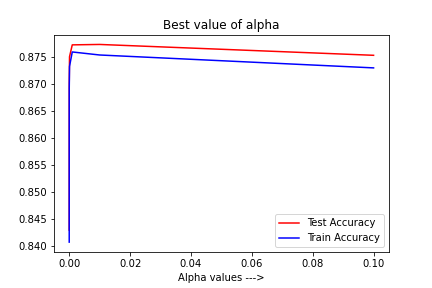
\includegraphics[width=250px]{SGD_complexity.png}
    \captionof{figure}{Complexity Curve: \emph{alpha} value for SGD}
\end{center}

\subsubsection{Model Evaluation}

With \emph{alpha}=0.01 we plotted a learning curve for the model as the sample size grows.
\begin{center}
    \captionsetup{type=figure}
    
\includegraphics[width=250px]{SGD Learning Curve.png}
    \captionof{figure}{Learning Curve for SGD}
\end{center}
This model shows extremely low bias and variance, and an increasing validation score as the data increases.\\
It is also important to note that this model only took a few seconds to train, which makes it much faster to train than the equivalent linear SVM, and much better suited for very large data.


\subsection{Ensemble: Random Forest}
\subsubsection{Presentation}
Ensemble learning models combine results of multiple models to improve overall performance.\\
There are many different techniques in which to apply this concept, we will be using a RandomForestClassifier, which falls under the bagging ensemble techniques.\\
Bagging is simply the idea of splitting the data into subsets and training a model on each subset, then combining the results to achieve a more generalized result, a RandomForestClassifier uses Decision Trees as the internal models.

\subsubsection{Defining Parameters}
The data for training and validating is already defined by the Data Preparation step (80\% train, 20\% validation).\\
Representative parameters for the model are \emph{n\_estimators}, \emph{max\_features}, and \emph{max\_depth}.
\begin{itemize}
    \item \underline{n\_estimators}: The number of internal models used in the ensemble.
    \item \underline{max\_features}: The maximum number of features allowed for the split in each decision tree.
    \item \underline{max\_depth}: The maximum depth of each tree in the ensemble.
\end{itemize}
We trained an ensemble using a GridSearch over a few different values of these parameters to see if we can achieve a higher accuracy than the defaults.\\
We achieved 96.4\% accuracy with the parameters set to {'bootstrap': True, 'max\_depth': 50, 'max\_features': 10, 'n\_estimators': 200}, only a slightly (0.2\%) higher accuracy score than default parameters.
Tuning this model proved difficult as it was overfitting the data very fast, as we can see from this complexity curves over different values of \emph{n\_estimators} and \emph{max\_depth}. \\
\begin{center}
    \captionsetup{type=figure}
    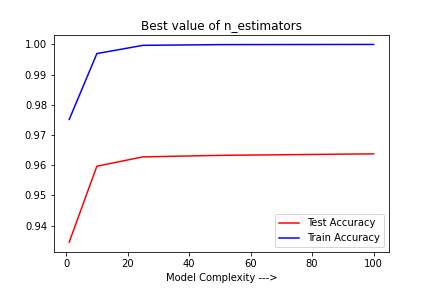
\includegraphics[width=250px]{RF_complexity_estimators.png}
    \captionof{figure}{Complexity Curve: \emph{n\_estimators} value for RFC}
\end{center}

\begin{center}
    \captionsetup{type=figure}
    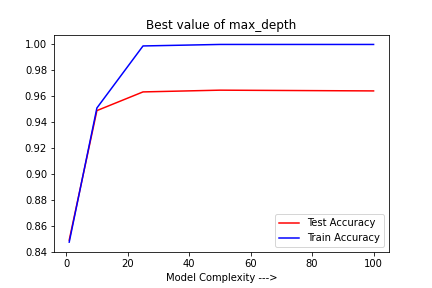
\includegraphics[width=250px]{RF_complexity_depth.png}
    \captionof{figure}{Complexity Curve: \emph{max\_depth} value for RFC}
\end{center}
\subsubsection{Model Evaluation}
We plotted the learning curve for the model using default params, over the training data split (around 90k rows).
\begin{center}
    \captionsetup{type=figure}
    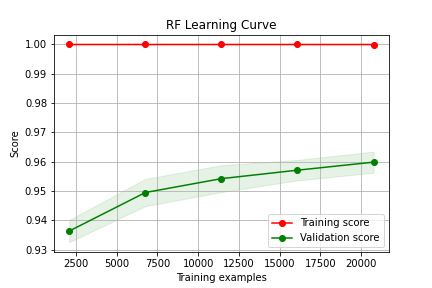
\includegraphics[width=250px]{learning_curve_RF_small.png}
    \captionof{figure}{Learning Curve for RFC over large dataset}
\end{center}
It shows a very high bias and an almost immediate overfitting, so as an experiment we plotted the learning curve over a smaller data split (in this case our validation split, about 30k rows) it showed how quickly the model overfits the training data.
\begin{center}
    \captionsetup{type=figure}
    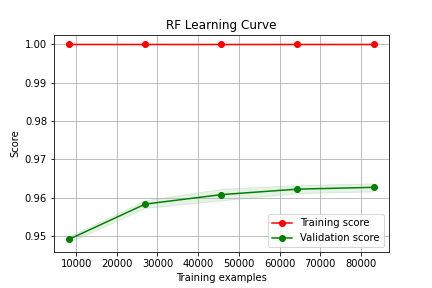
\includegraphics[width=250px]{learning_curve_RF_big.png}
    \captionof{figure}{Learning Curve for RFC over small dataset}
\end{center}

\subsection{Voting Classifier}
\subsection{Presentation}
The Voting Classifier is an ensemble model which provides a classification using many other classification models.
In this case, we use all previously trained and tuned models as input to a Voting Classifier

\subsection{Input Models}
\begin{itemize}
    \item K-Nearest-Neighbors: \emph{k = 5}
    \item Decision Tree: \emph{maximum depth = 13}
    \item Support Vector Machine: \emph{gamma = 0.03 ; C = 0.8}
    \item Neural Network (MLP): \emph{alpha = 0.001 ; learning rate (constant) = 0.005}
    \item Stochastic Gradient Descent: \emph{alpha = 0.01}
    \item Random Forest: \emph{max\_depth = 20}
\end{itemize}

\subsubsection{Model Evaluation}
The learning curve shows us the training and validation scores for different data sizes.\\
This way, we are able to say that the score is bounded below 97.5\%, and the model doesn't seem to continue learning after 80000 training rows.
\begin{center}
    \captionsetup{type=figure}
    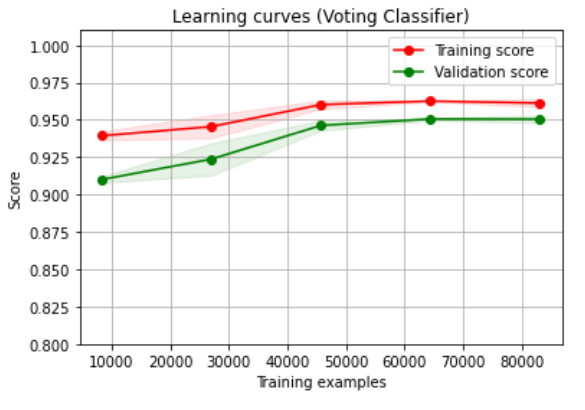
\includegraphics[width=250px]{learning_curve_voting.png}
    \captionof{figure}{Learning Curve for Voting Classifier}
\end{center}


\section{AUCs}

\section{AutoML}
% (+ new AUC, including AUC)

\section{Best model: model n}
% TODO: complete model
% Why the best
\subsection*{PCA}
% Does it improve?

\section*{Conclusion}
\addcontentsline{toc}{section}{Conclusion}
After evaluating nine classifier models, including two ensembles and a model given by AutoML,
we find as our best option for predicting Airline Passenger Satisfaction the Voting Classifier,
with five different classifiers as inputs (KNN, Decision Tree, SVM, MLP and Stochastic Gradient Descent),
each one of them with their tuned parameters.\\
Although this is an extensive study, possibilities are much more and (most likely) outperforming our choice (as a starting point for future work, we propose increasing the size of the dataset, and retrain Neural Network and Stochastic Gradient Descent models).
Also, batch-processing done during this research is not as demanding as more complex Machine Learning technologies
(deeper Neural Networks, more complex ensembles, etc.). There's still much work to do.


\end{document}
